\documentclass{article}
\usepackage[utf8]{inputenc}
\usepackage{graphicx}
\usepackage{amsmath, amsthm, amssymb}
\usepackage{multicol}
\usepackage{svg}
\usepackage{caption}
\usepackage{vmargin}
\usepackage[hidelinks]{hyperref}
\usepackage[utf8]{inputenc}
\usepackage{epigraph}

\theoremstyle{definition}
\newtheorem{defi}{Definition}[section]
\newtheorem{theorem}{Theorem}[section]
\newtheorem{prop}{Properties}[section]
\newtheorem{lemma}{Lemma}[section]

\usepackage{mathtools}
\DeclarePairedDelimiter\ceil{\lceil}{\rceil}
\DeclarePairedDelimiter\floor{\lfloor}{\rfloor}

\title{Probability Distributions}
\author{Xiaozhe Yao\footnote{https://yaonotes.org/lecture-notes}}
\date{\today}
\begin{document}

\maketitle

\section{Basic Concepts}

\begin{defi}
\textbf{Probability Distribution} In probability theory and stats, a probability distribution is a mathematical function that provides the probabilities of occurrence of different possible outcomes in an experiment. More technically, the probability distribution is a description of a random phenomenon in terms of the probabilities of events.
\end{defi}

\begin{defi}
\textbf{Sample Space} A probability distribution is specified in terms of an underlying \textit{sample space}, which is the set of all possible outcomes of the random phenomenon being observed. 
\end{defi}

\begin{defi}
\textbf{Types of Distribution} 

By different outcomes, probability distributions are generally divided into two classes:\begin{itemize}
    \item \textit{Discrete Probability Distribution}, where the set of possible outcomes is discrete and can be encoded by a discrete list of the probabilities of the outcomes, known as a probability mass function (PMF).
    \item \textit{Continuous Probability Distribution}, where the set of possible outcomes can take on values in a continuous range, and is typically described by probability density functions (with the probability of any individual outcome actually being 0).
\end{itemize} 

By different sample spaces, probability distributions can be divided into the following types:
\begin{itemize}
    \item \textit{Univariate}: Sample Space is one dimensional, such as real numbers, list of labels, ordered labels or binary. It gives the probabilities of a single random variable taking on various alternative values.
    \item \textit{Multivariate}: Sample space is a vector space of dimension $2$ or more. It gives the probabilities of a random vector - a list of two or more random variables.
\end{itemize}
\end{defi}

\begin{defi}
\textbf{Cumulative Distribution Function (CDF)} The CDF of a real-valued random variable $\textbf{X}$, or just the distrbution function of $\textbf{X}$, evaluated at $x$, is the probability that $\textbf{X}$ will take a value less than or equal to $x$.
\end{defi}

\section{Bernoulli Distribution}
\begin{defi}
\textbf{Bernoulli Distribution} is a discrete probability distribution of a random variable which takes the value $1$ with probability $p$ and the value $0$ with probability $q=1-p$.
\end{defi}
\begin{prop} There are some fundamental facts for Bernoulli Distribution:
\begin{itemize}
    \item If $\textbf{X}$ is a random variable with this distribution, then $$Pr(X=1)=p=1-Pr(X=0)=1-q$$.
    \item The probability mass function $f$ of this distribution, over possible outcomes $k$, is $$f(k;p)=\begin{cases}
               p & \text{if k=1}\\
               1-p & \text{if k=0} \\
            \end{cases}$$ It can be expressed as $$f(k;p)=p^k(1-p)^{(1-k)}, k\in\{0,1\}$$ or as $$f(k;p)=pk+(1-p)(1-k)$$
    \item The expectation $E(X)=\sum_{x}xP(X=x)=1\times p + 0\times (1-p)=p$.
    \item The variance is $Var(X)=p(1-p)$. To prove, simply plug $E(X)$ in it: $Var(X)=E(X^2)-E(X)^2=p-p^2=p(1-p)$.
\end{itemize}
\end{prop}
\begin{theorem}
\textbf{The expectation and variance theorem}. Assume $X,Y$ are two independent variables.
    \begin{itemize}
        \item $E(XY)=E(X)E(Y)$.
        \item $Var(X+Y)=Var(X)+Var(Y)$.
    \end{itemize}
\begin{proof}
As below:
\begin{itemize}
    \item $E(XY)=xy\sum_{x}\sum_{y}P(X=x, Y=y)$, as $X,Y$ are independent to each other, $$P(X=x,Y=y)=P(X=x)P(Y=y)$$ thus $$\sum_{x}\sum_{y}xyP(X=x, Y=y)=\sum_{x}xP(X=x)\sum_{y}yP(Y=y)=E(X)E(Y)$$
    \item $Var(X+Y)\\=E((X+Y)^2)-E(X+Y)^2\\=E(X^2+2XY+Y^2)-(E(X)+E(Y))^2\\=E(X^2)+E(Y^2)+2E(XY)-E(X)^2-E(Y)^2-2E(X)E(Y)$, 
    
    by using the fact that $E(XY)=E(X)E(Y)$, we continue
    
    $Var(X+Y)\\=E(X^2)-E(X)^2+E(Y^2)-E(Y)^2\\=Var(X)+Var(Y)$.
\end{itemize}
\end{proof}
\end{theorem}

\textit{Note:} Bernoulli Distribution is a special case of binomial distribution, with $n=1$.

\section{Binomial Distribution}

\begin{defi}
\textbf{Binomial Distribution}. Binomial Distribution with parameters $n$ and $p$ is the discrete probability distribution of the number of successes in a sequence of $n$. Each asking a single yes/no question and gives boolean-valued outcome. That is, A single experiment is a \textit{Bernoulli experiment}, or named \textit{Bernoulli trial}. A sequence of outcomes is called a Bernoulli process. 

If the random variable $X$ follows the binomial distribution with parameters $n\in \mathbb{N}$ and $p\in[0,1]$, we write it as $X\sim B(n,p)$.
\end{defi}

\begin{prop}
\textbf{PMF} The probability of getting exactly $k$ successes in $n$ independent Bernoulli trials is given by the probability mass function: $$f(k,n,p)=Pr(k;n,p)=Pr(X=k)=C_{n}^{k}p^k(1-p)^{n-k}, \: C_{n}^{k}=\frac{n!}{k!(n-k)!}$$

The formula can be understood as: $k$ successes occur with probability $p^k$ and $n-k$ failures occur with probability $(1-p)^{n-k}$. Then the successes can occur anywhere among the $n$ trials, and therefore there are $C_{n}^{k}$ different ways of distributing $k$ successes in a sequence of $n$ trials.

\textbf{Monotonicity} There is always an integer M such that $f(k,n,p)$ is monotone increasing for $k<M$, and monotone decreasing for $k>M$
When calculating the PMF, we can safely calculate only $\frac{n}{2}$, by the definition of binomial coefficients, we have $f(k,n,p)=f(n-k,n,1-p)$.

\begin{figure}[h]
\caption{Probability Mass Function for Binomial Distribution}
\centering
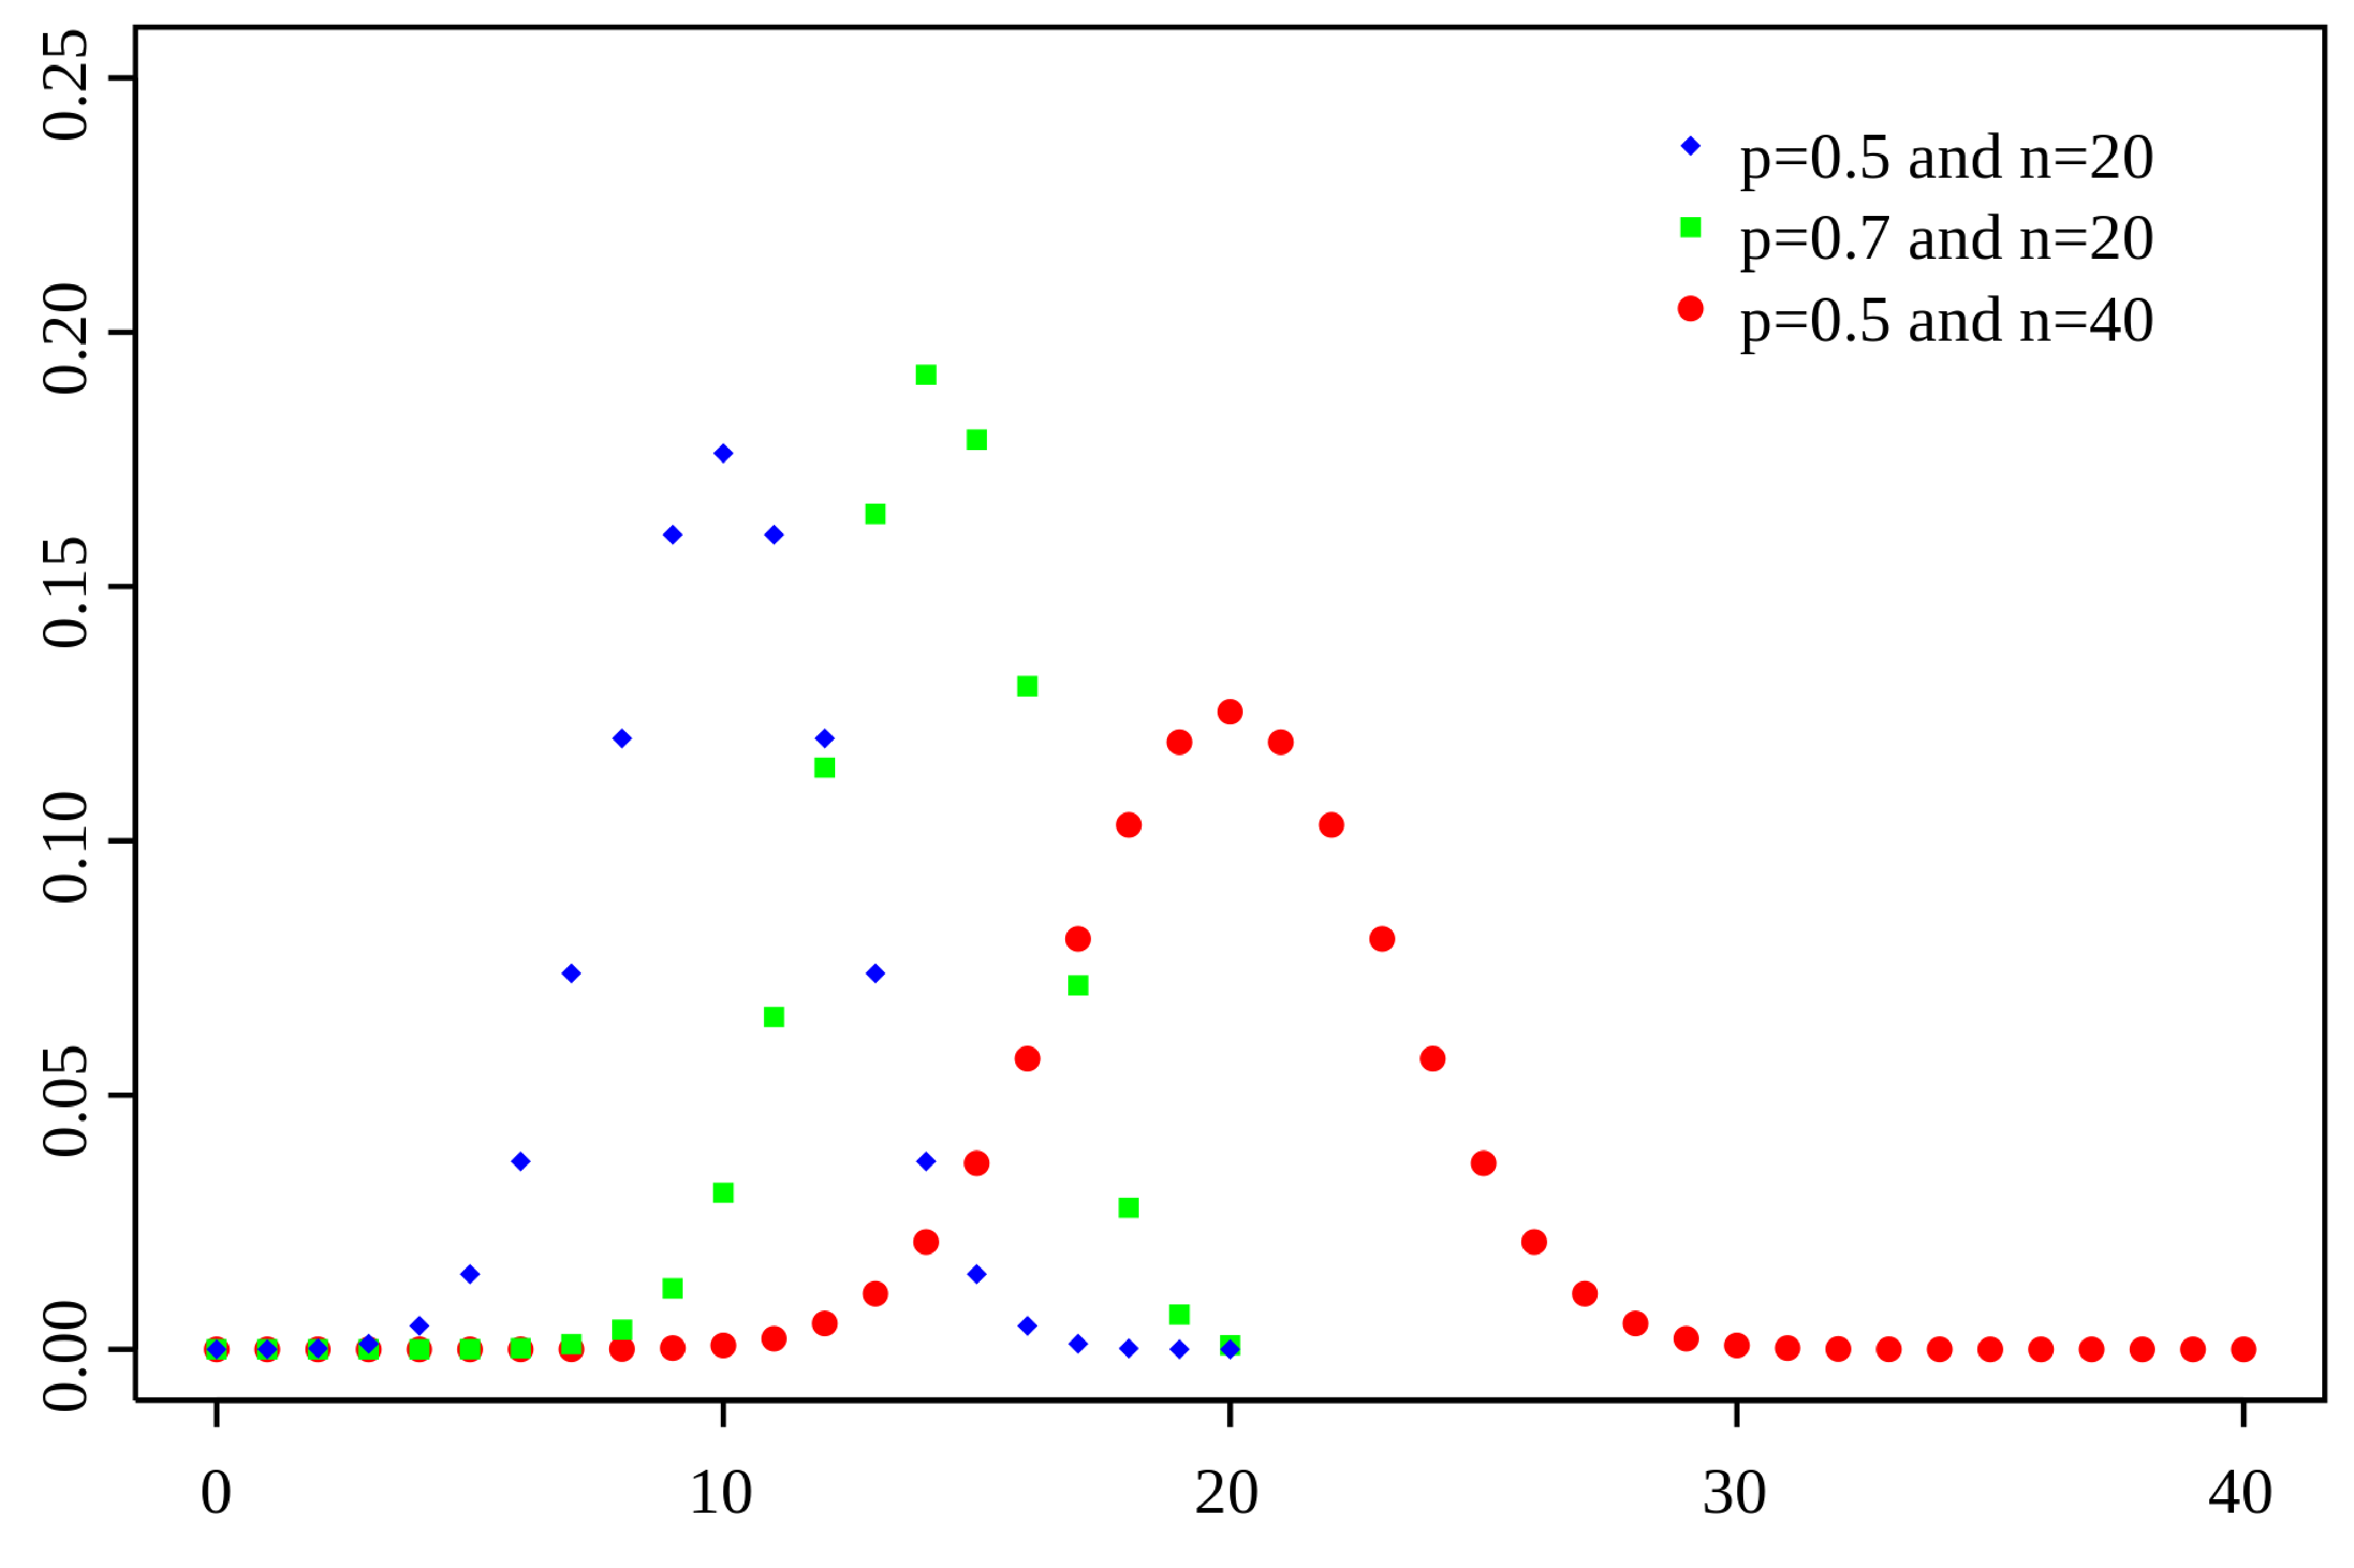
\includegraphics[width=\textwidth]{Statistics/images/Binomial_distribution_pmf.pdf}
\end{figure}

\end{prop}

\begin{prop}
\textbf{CMF} The cumulative distribution function can be expressed as $F(k,n,p)=Pr(X\leq k)=\sum_{i=0}^{\floor*{k}}C_{n}^{i}p^i(1-p)^{n-i}$, where $\floor*{k}$ refers to the greatest integer less than or equal to $k$.
\begin{figure}[h]
\caption{Cumulative Distribution Function for Binomial Distribution}
\centering
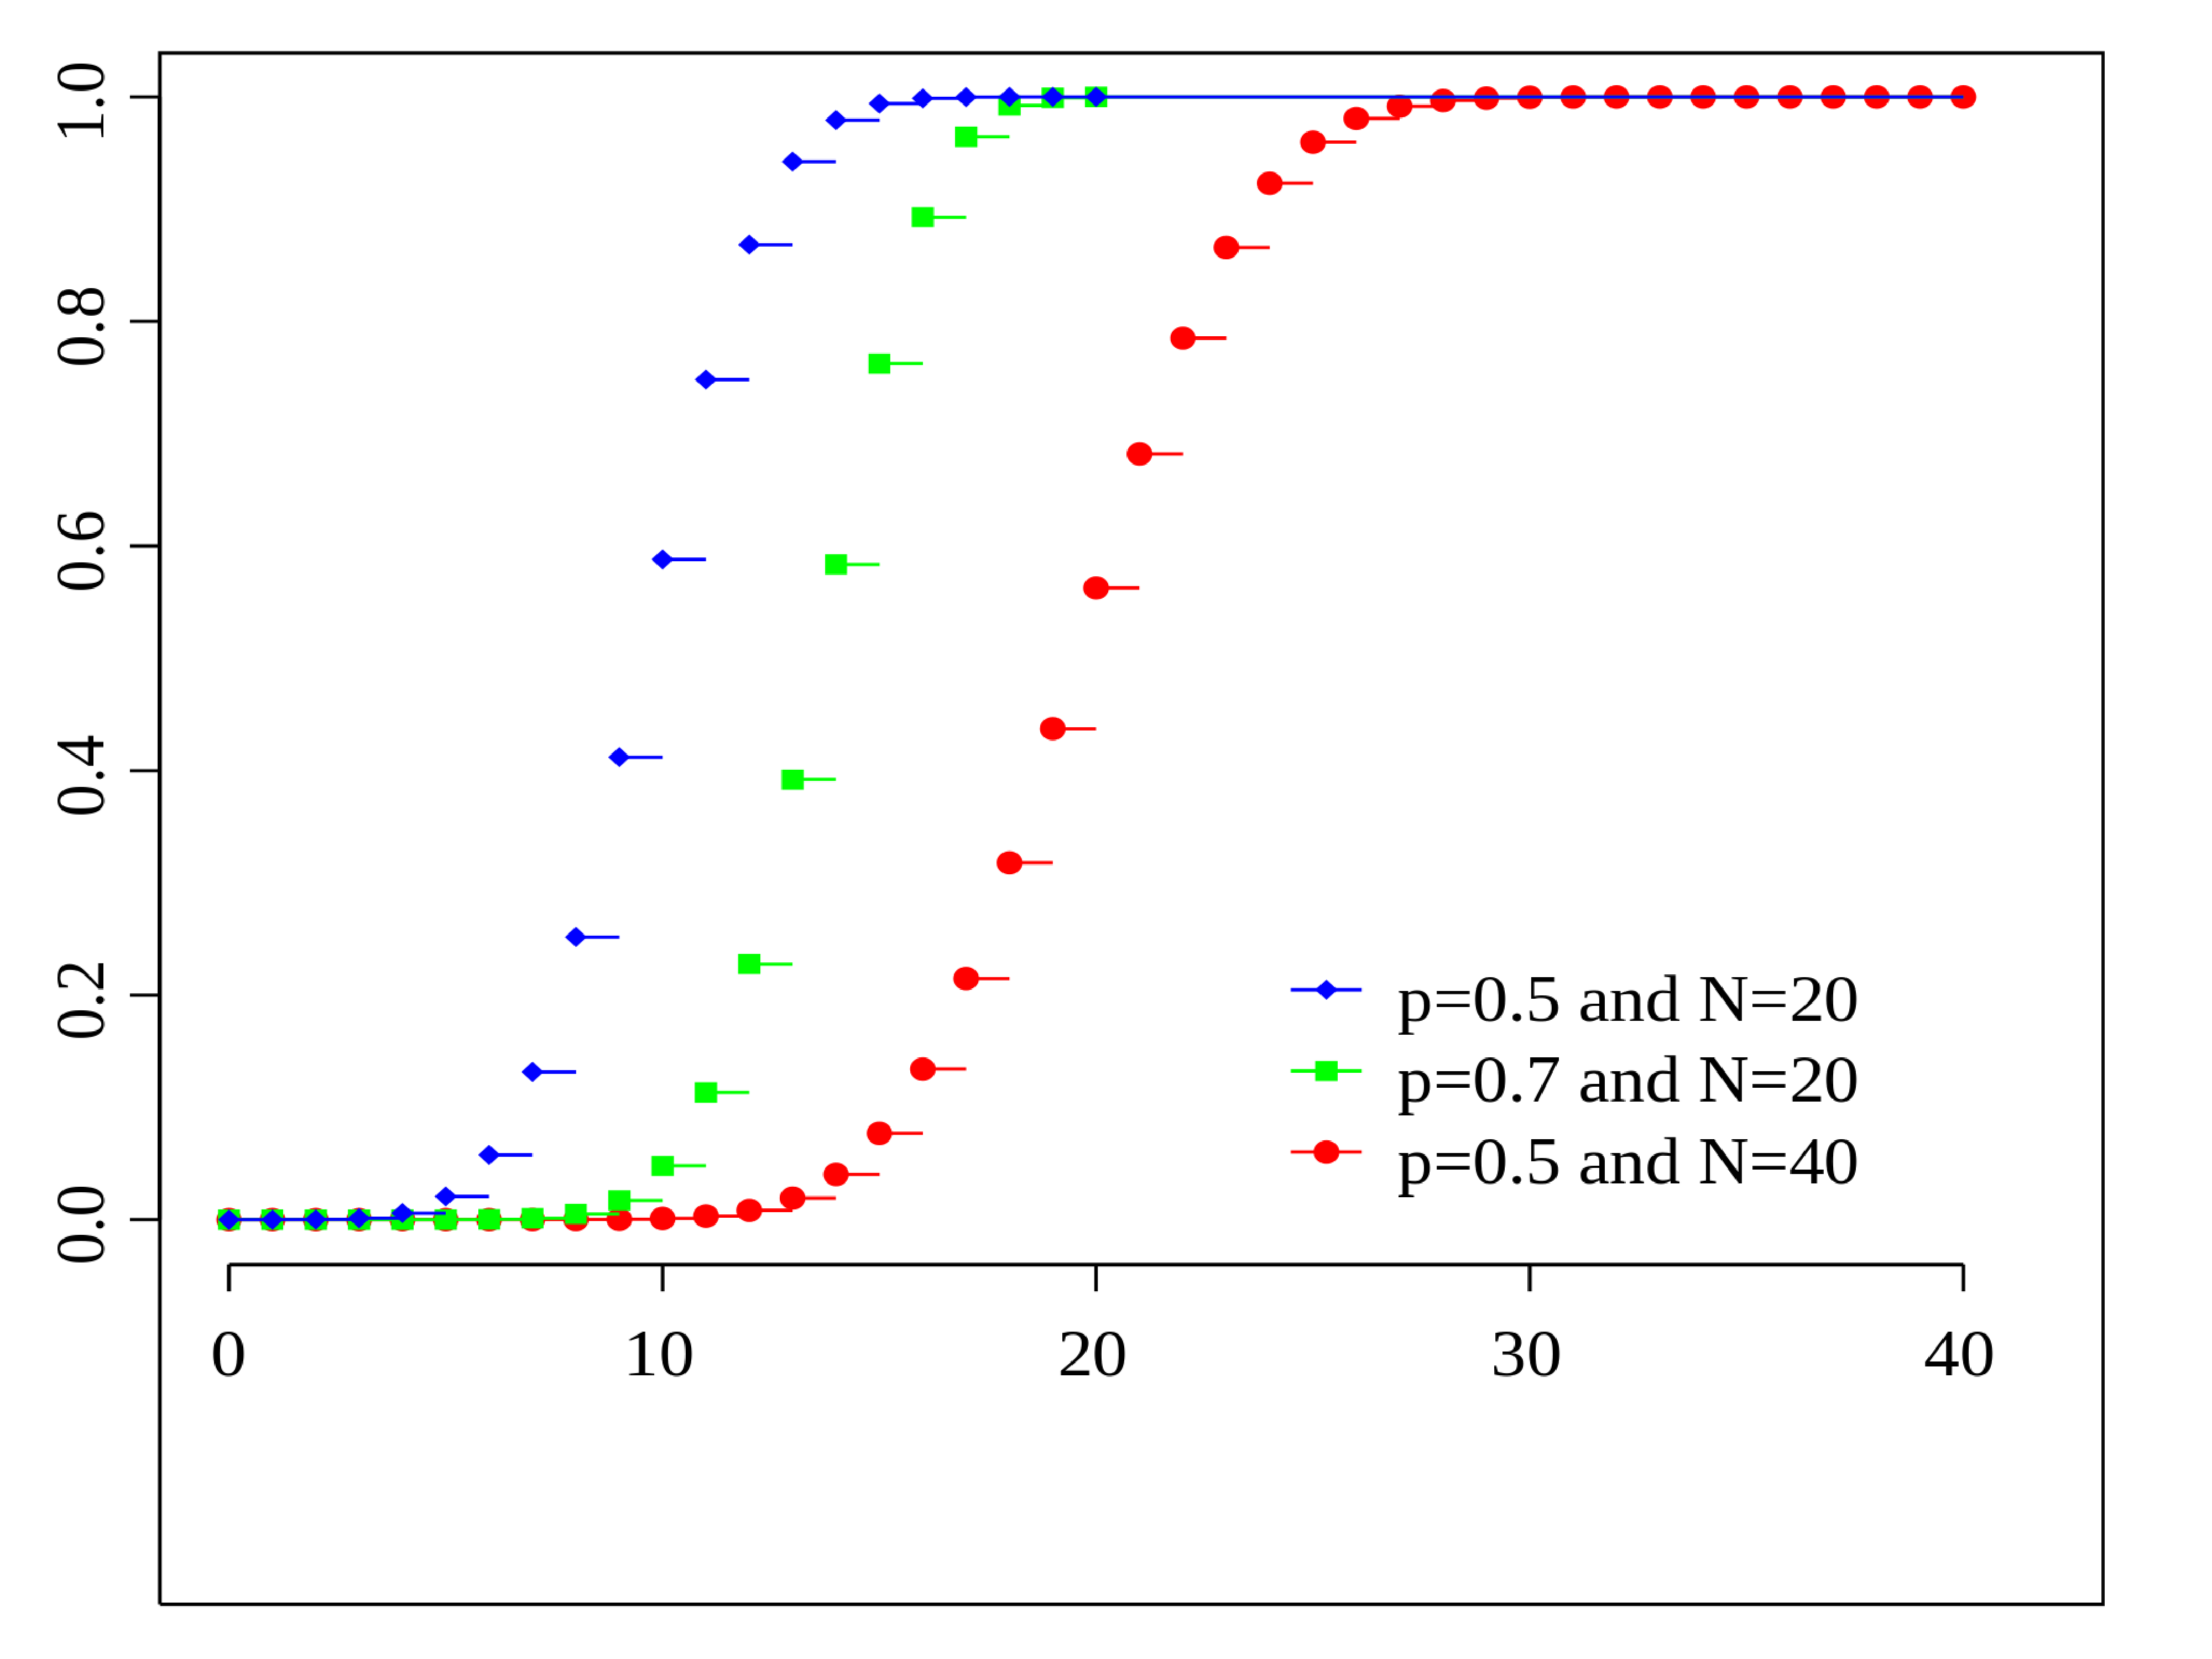
\includegraphics[width=\textwidth]{Statistics/images/Binomial_distribution_cdf.pdf}
\end{figure}

\end{prop}
\begin{prop}
\textbf{Expectation} If $X\sim B(n,p)$, then $E(X)=np$.
\begin{proof}
This follows from the linearity of the expected value along with fact that $X$ is the sum of $n$ identical, independent Bernoulli random variables, each with expected value $p$, i.e. $X=X_1+X_2+...+X_n=\sum_{i=1}^{n}X_i$. Thus $E(X)=E(\sum_{i=1}^{n}X_i)=E(X_1+...+X_n)=E(X_1)+...E(X_n)=\sum_{i=1}^{n}E(X_i)=\sum_{i=1}^{n}p=np$.
\end{proof}
\end{prop}

\begin{prop}
\textbf{Variance} If $X\sum B(n,p)$, then $Var(X)=np(1-p)$.
\begin{proof}
It also follows from the fact that the variance of a sum of independent random variables is the sum of the variances.
$Var(X)=Var(\sum_{i=1}^{n}X_i)=Var(X_1+...+X_n)=Var(X_1)+...+Var(X_n)=\sum_{i=1}^{n}Var(X_i)=np(1-p)$.
\end{proof}
\end{prop}

\subsection{Hypergeometric Distribution}

In Binomial Distribution, every trial is independent to each other. In some cases, the previous trials may have some impact on the future trials. For example, there are $n$ objects, and $k$ objects with the property $\mathcal{P}$, we take the objects randomly, then the probability for ``get an object with the property $\mathcal{P}$" is $p=\frac{k}{n}$. We do this experiment one by one.
\begin{itemize}
    \item If we return the object everytime we complete a single trial, then every trial is identical and independent to each other. It is binomial distribution.
    \item If we \textbf{DONT} return, then every trial will not be independent and identical, and in this case it is called hypergeometric distribution.
\end{itemize}

\begin{defi}
\textbf{Hypergeometric Distribution} Hypergeometric Distribution is a discrete probability distribution that describes the probability of $k$ successes (random draws for which the object drawn has a specified feature) in $n$ draws, \textbf{without replacement}. The process is from a finite population size $N$ that contains $K$ objects with that feature.
\end{defi}

\begin{prop}
\textbf{PMF} The following conditions characterize the hypergeometric distribution:
\begin{itemize}
    \item The result of each draw is binary.
\end{itemize}
\end{prop}

\section{Poisson Distribution}

\section{Normal Distribution}
\end{document}